\subsection{Command-Service}
\label{subsec:implementation:commandService}
 Ähnlich wie beim \textit{Query-Service}, wird auch beim \textit{Command-Service} für jeden ankommenden Befehl ein eigener Actor gestartet, welcher für diesen speziellen Typ von Anfrage zuständig ist. Es gibt auch hier für jeden möglichen Befehl einen eigenen Actor welcher die Logik des Kommandos beinhaltet. Jedoch werden in der Implementierung der einzelnen Kommandos meist neue Befehle an einen oder mehrere zuständige Actors aus dem Domain-Service erzeugt und weitergeleitet. \\
 In der vorliegenden Implementierung gibt es folgende unterschiedliche Typen von Kommandos, welche alle durch einen \textit{CommandHandler} repräsentiert werden:
 \begin{enumerate}
     \item Flüge erstellen
     \item Flug Vorbereiten
     \item Ticket Reservieren
     \item Ticket Buchen
 \end{enumerate}
Die Abbildung \ref{fig:implementation:commandActorModel} zeigt den Aufbau des \textit{Command-Service}, welcher ähnlich zum Aufbau des \textit{Query-Service} ist. Die eigentliche Geschäftslogik ist jedoch in den Actoren des \textit{Domain Serice} beherbergt. Somit ist die Tätigkeit der einzelnen \textit{CommandHandler} darauf begrenzt, die betroffenen Actoren im \textit{Domain Serice} über die gewünschte Tätigkeit zu Informieren und diese auch auszuführen. 
 \begin{figure}
    \centering
    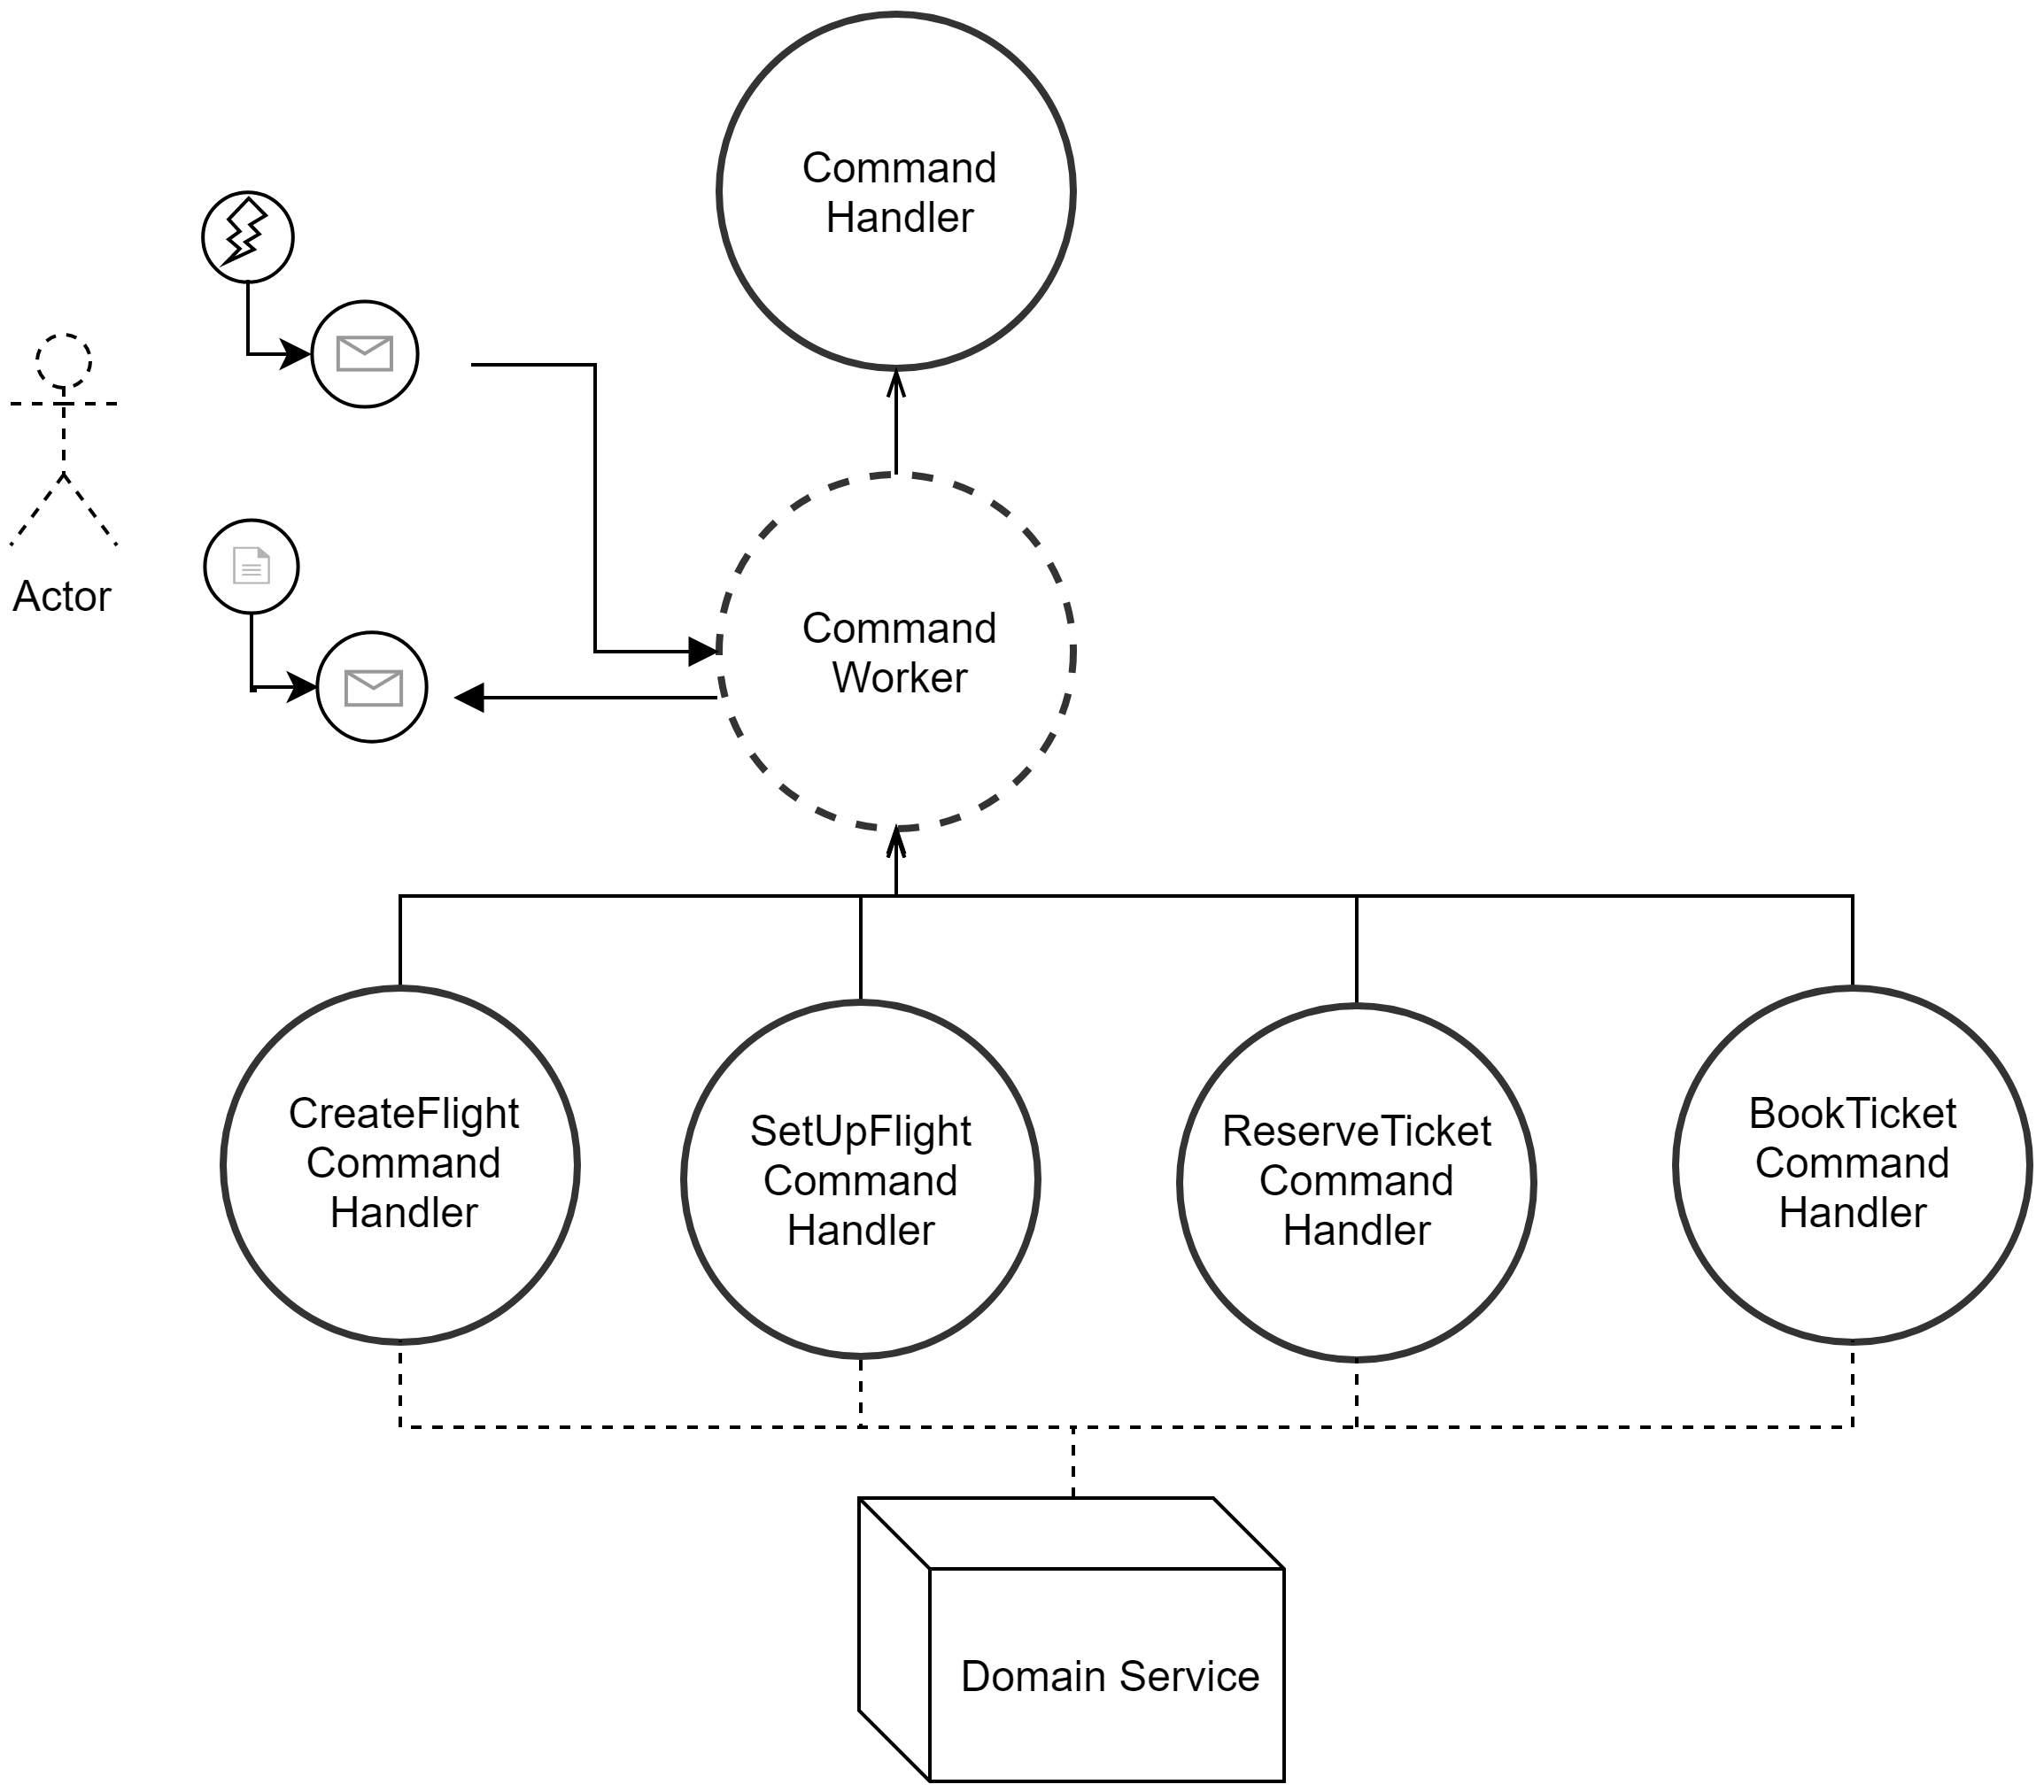
\includegraphics[width=0.8\linewidth]{gfx/implementation/CommandServiceActorModel}
    \caption{Der Aufbau des \textit{Command-Service} beinhaltet die Logik der einzelnen Befehle und leitete weitere Befehle an den \textit{Domain-Service} weiter }
    \label{fig:implementation:commandActorModel}
\end{figure} 

